% \chapter{The first appendix}

% Text for the first appendix goes here.

% \section{Appendix section}

% Text for a section in the first appendix goes here.

% test ทดสอบฟอนต์ serif

% \textsf{test ทดสอบฟอนต์ sans serif}

\ifenglish\else
% TODO: Thai teletype font still doesn't work with english option
% \verb+test ทดสอบฟอนต์ teletype ภาษาไทย+

% \texttt{test ทดสอบฟอนต์ teletype ภาษาไทย}
\fi

\chapter{\ifenglish Manual\else คู่มือการใช้งานระบบ\fi}

%
เมื่อนักศึกษาเข้ามาที่เว็บแอพพลิเคชันจะพบกับหน้า Home
\begin{figure}[h]
  \begin{center}
    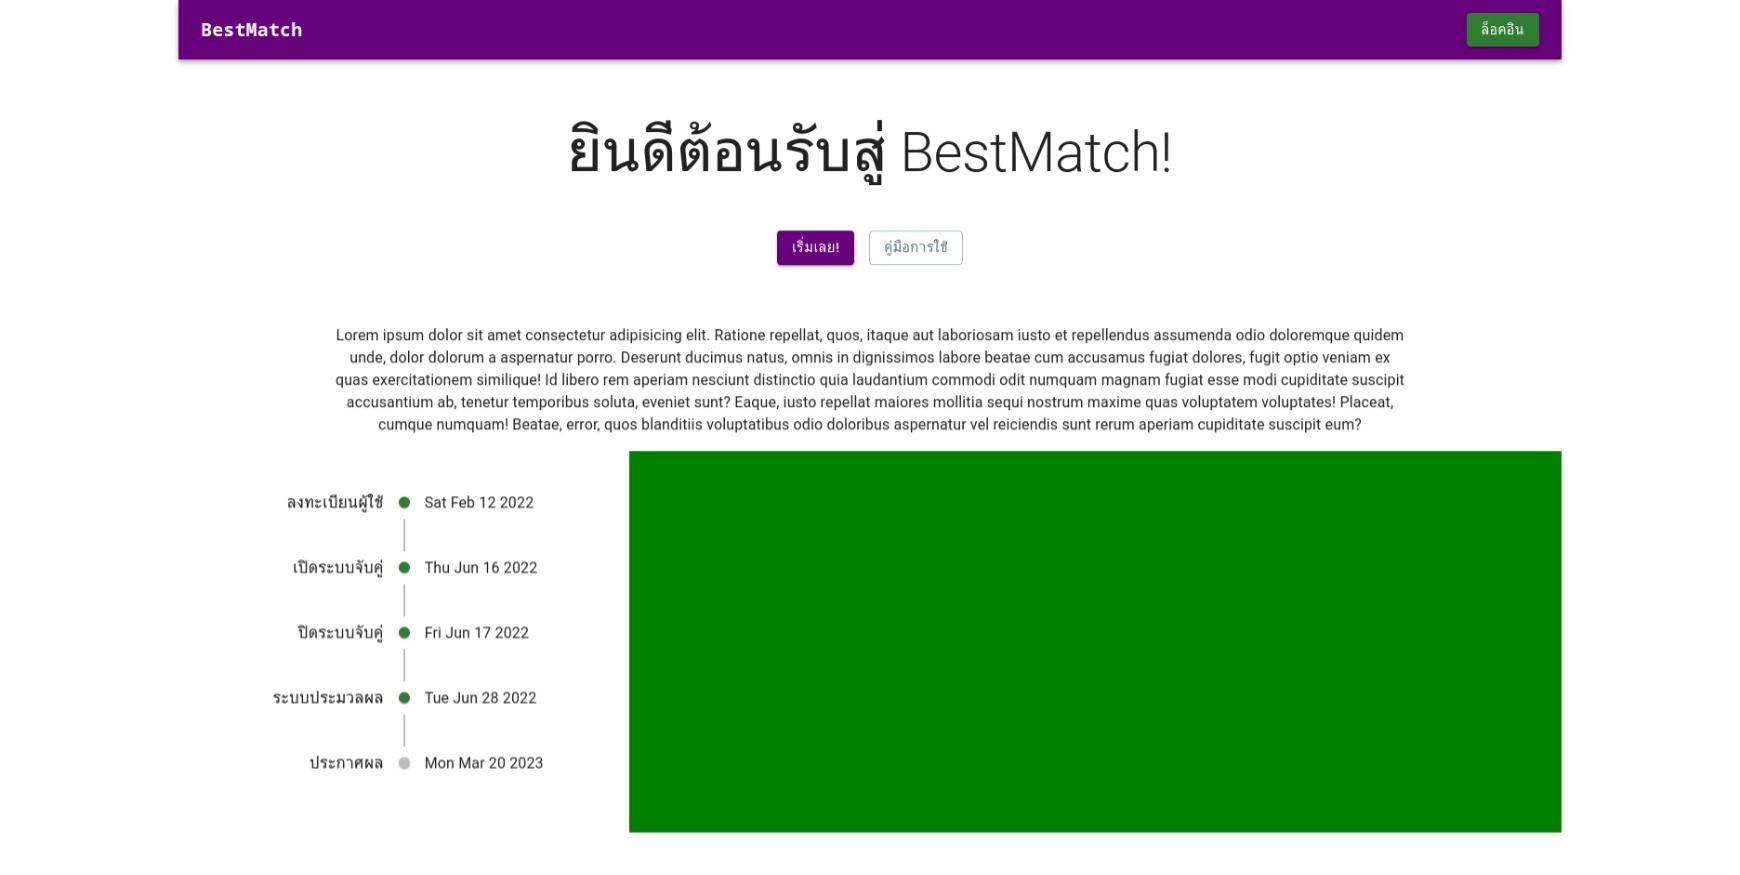
\includegraphics[width=\linewidth]{photo/web/student/home.jpeg}
  \end{center}
  \caption{หน้า Home}
\end{figure}
%
\newline
หลังจากนั้นจะกดปุ่ม "ล็อคอิน" หรือ "เริ่มเลย!" เพื่อทำการลงชื่อเข้าใช้
\begin{figure}[ht]
  \begin{center}
    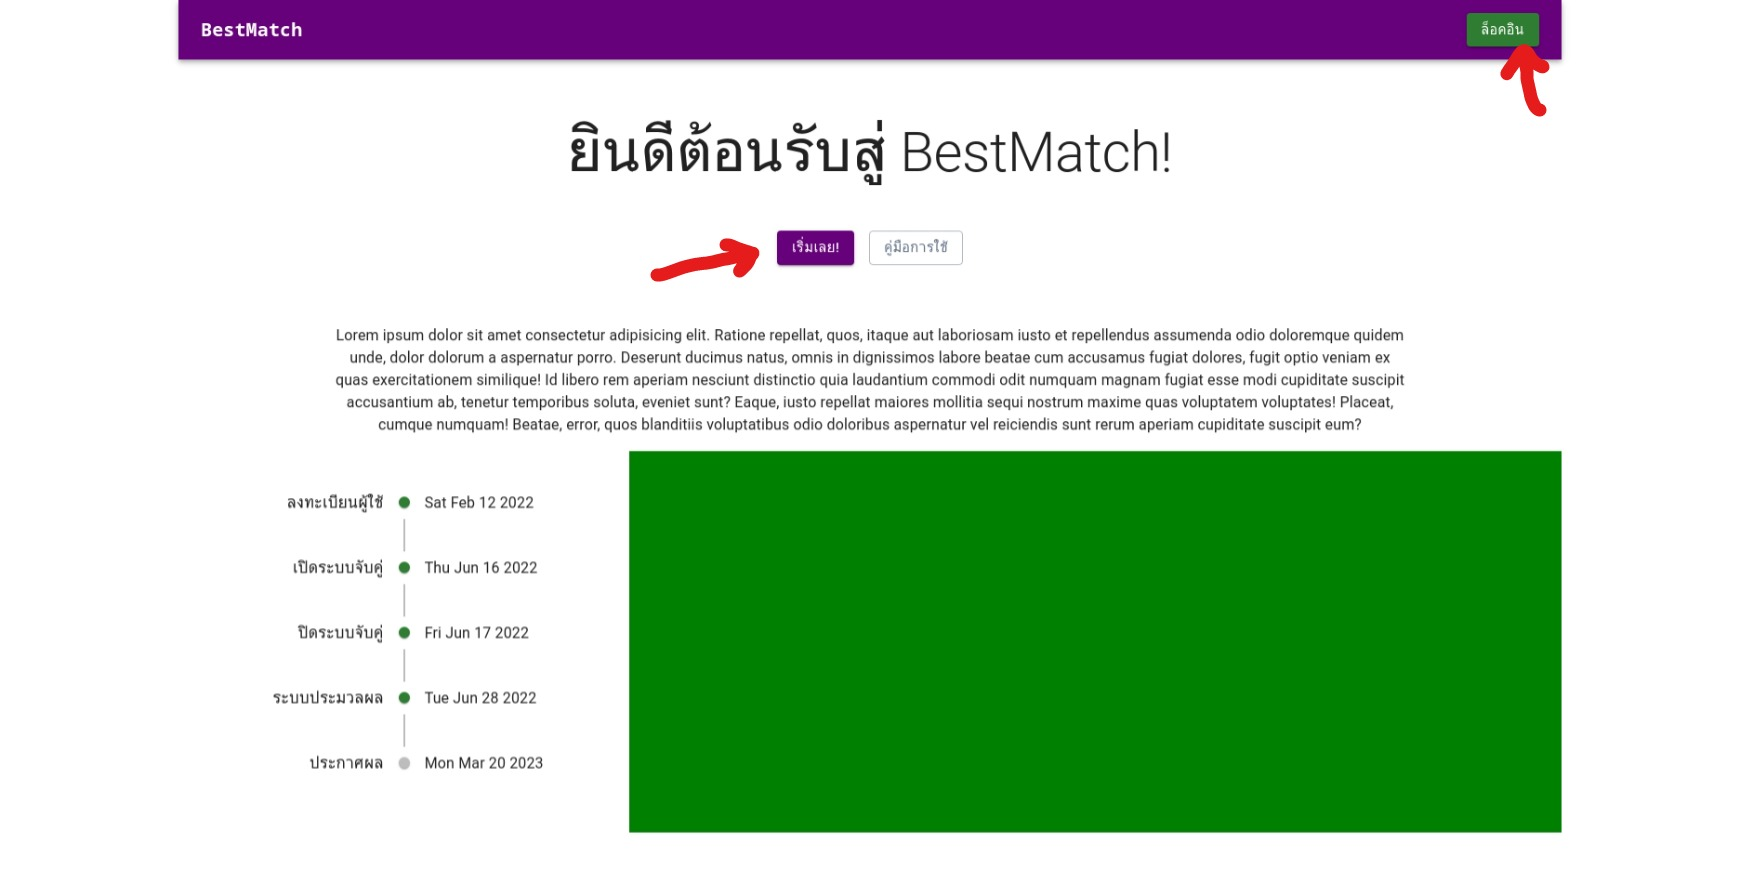
\includegraphics[width=\linewidth]{photo/web/student/login-btn.jpeg}
  \end{center}
  \caption{รูปตัวอย่างแสดงตำแหน่งปุ่ม "ล็อคอิน" และ "เริ่มเลย!"}
\end{figure}
\newpage 

หลังจากนั้นกรอกข้อมูลที่ใช้ในการยืนยันตัวตนในการเข้าใช้งาน
\begin{figure}[!ht]
  \begin{center}
    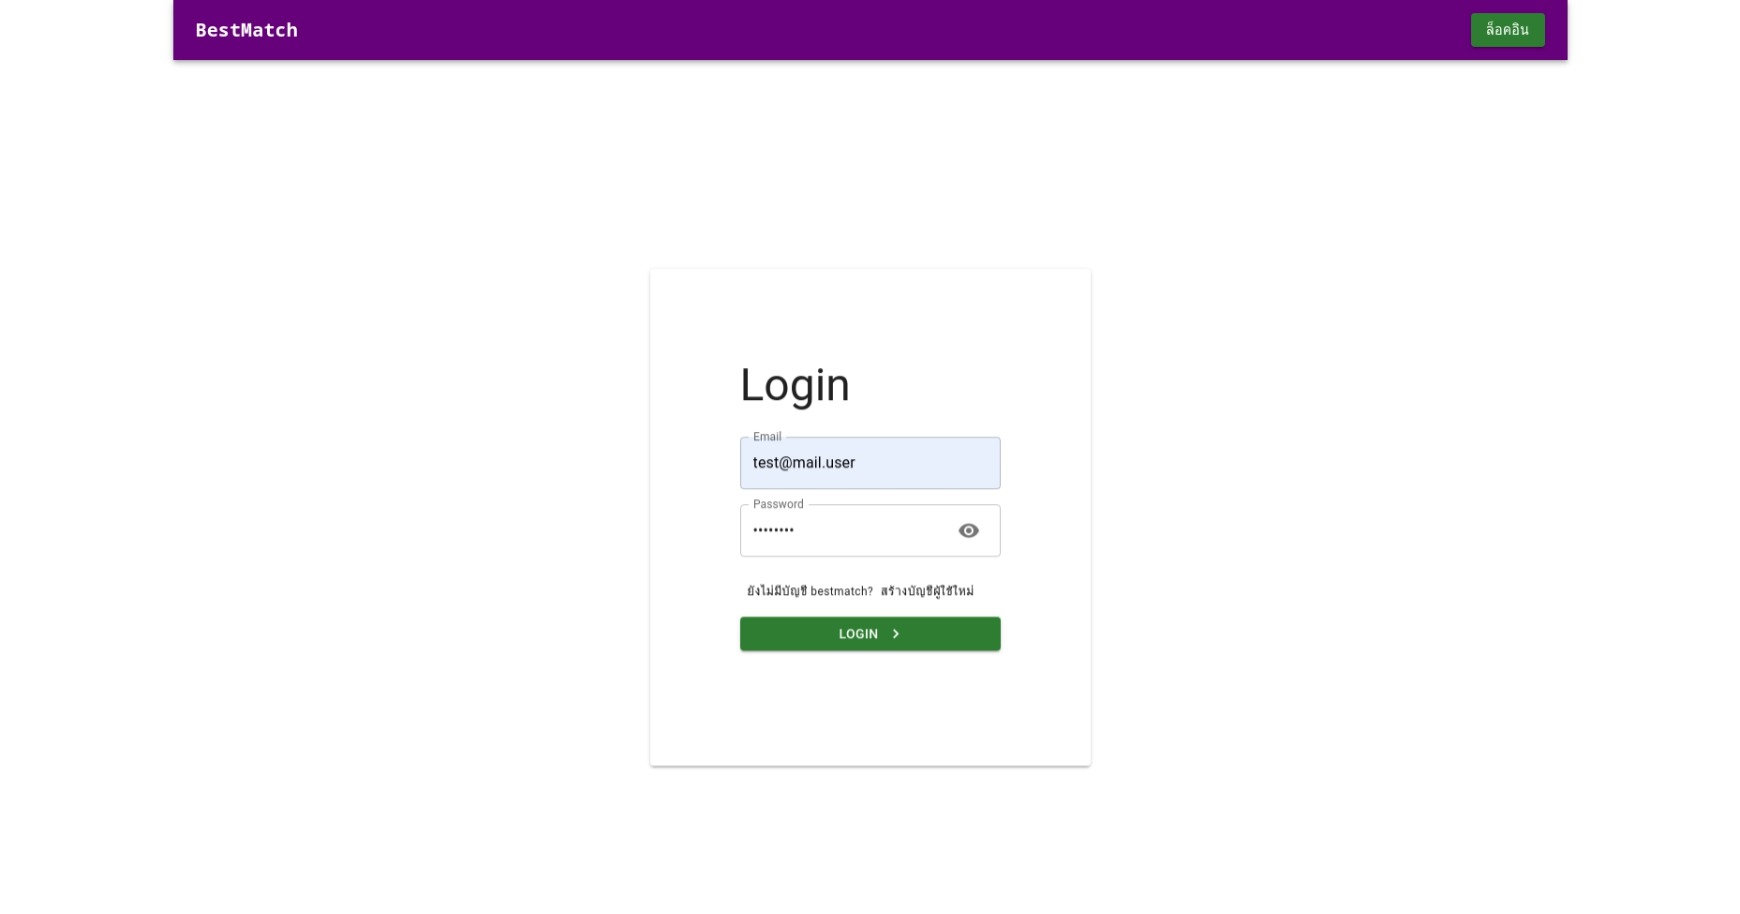
\includegraphics[width=\linewidth]{photo/web/student/login.jpeg}
  \end{center}
  \caption{หน้า Login}
\end{figure}
%
\newline
หากยังไม่มีบัญชีผู้ใช้จะต้องทำการสร้างบัญชีผู้ใช้โดยคลิกที่ "สร้างบัญชีผู้ใช้ใหม่"
\begin{figure}[!ht]
  \begin{center}
    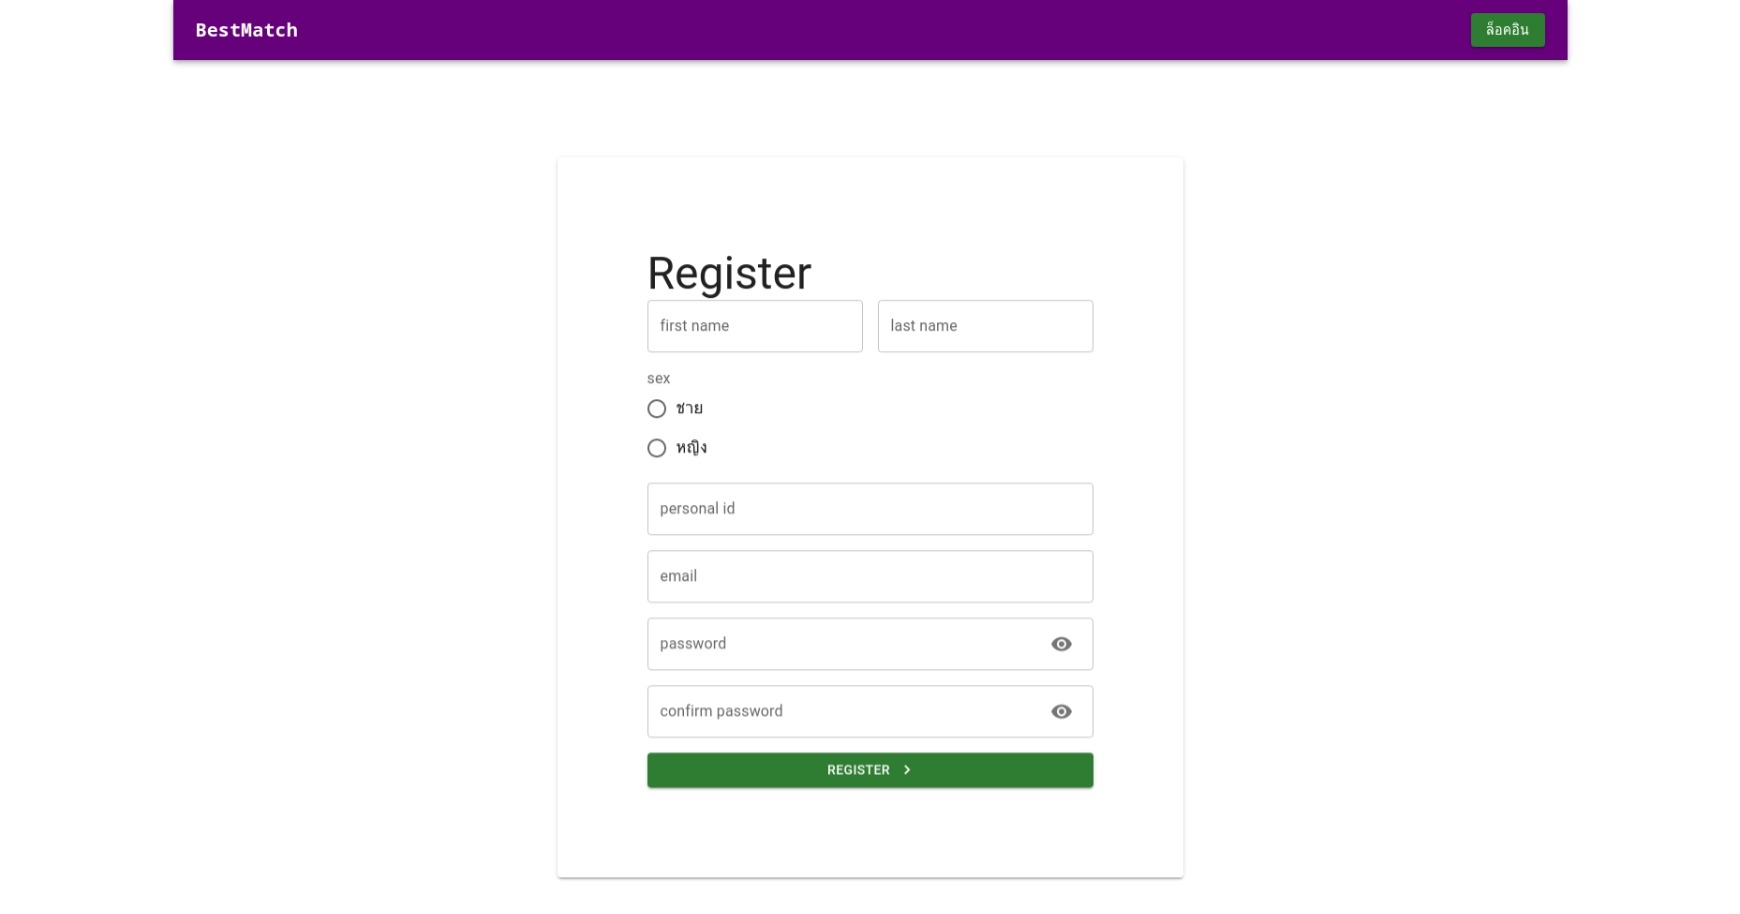
\includegraphics[width=\linewidth]{photo/web/student/register.jpeg}
  \end{center}
  \caption{หน้า Register}
\end{figure}
\newpage

เมื่อลงชื่อเข้าใช้แล้วจะกลับมาที่หน้า Home พร้อมกับอีเมล์ของผู้ใช้
\begin{figure}[!ht]
  \begin{center}
    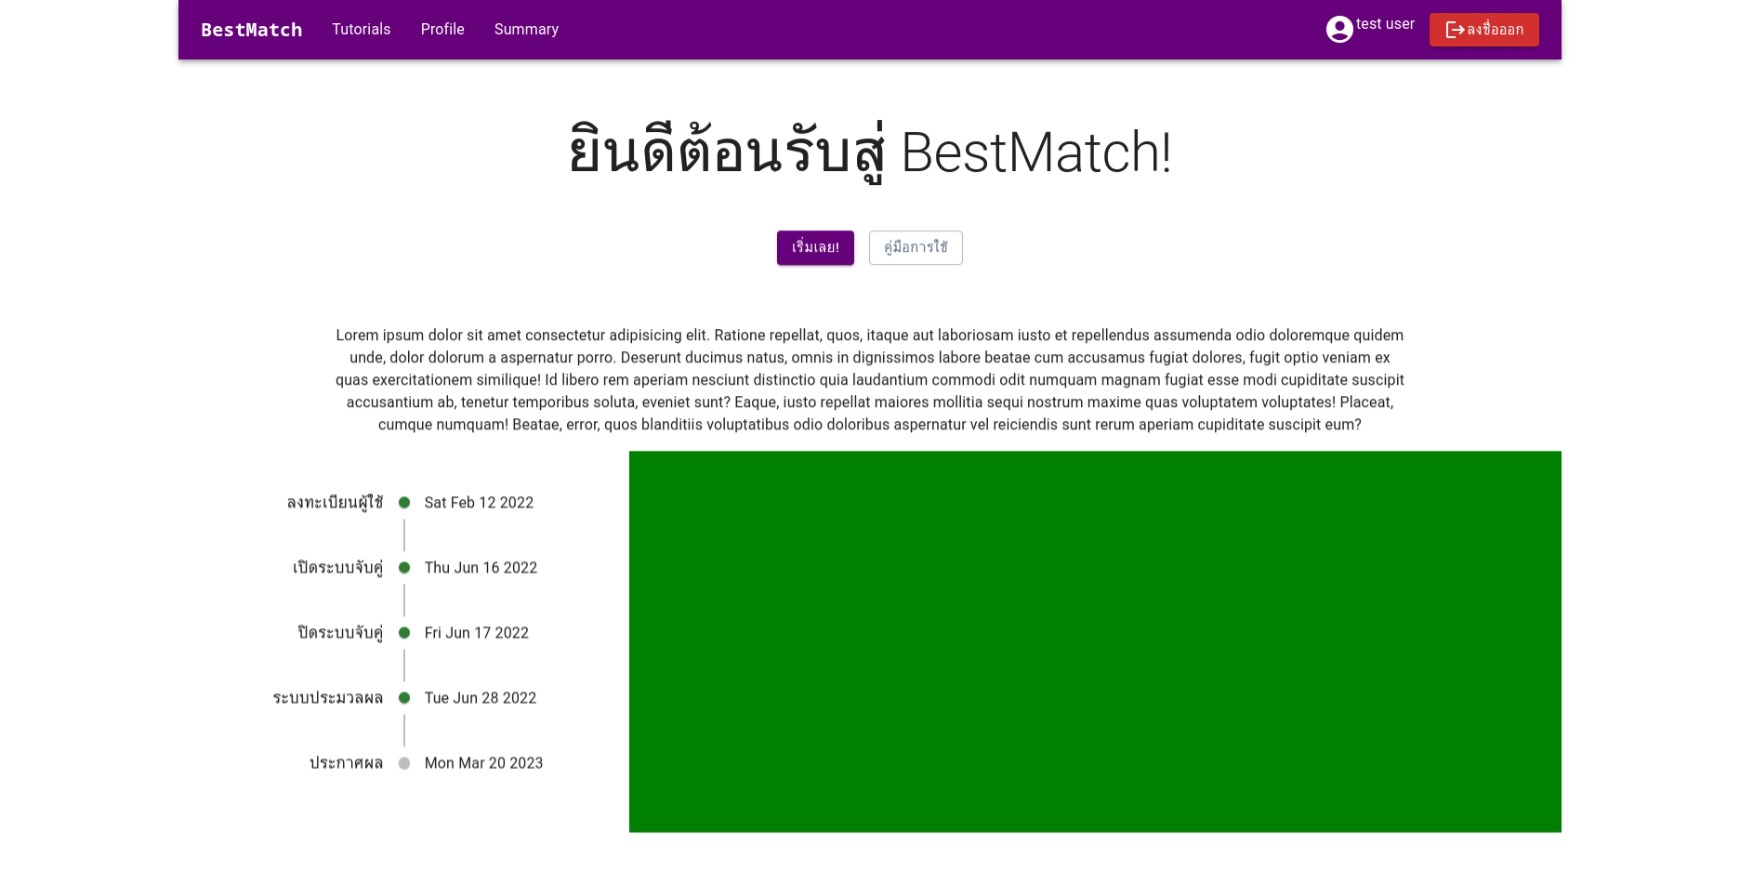
\includegraphics[width=\linewidth]{photo/web/student/home-auth.jpeg}
  \end{center}
  \caption{หน้า Home หลังยืนยันตัวตนสำเร็จ}
\end{figure}
%
\newline
เมื่อกดปุ่ม "เริ่มเลย" จะไปที่หน้าแอพพลิเคชันหลัก ซึ่งจะให้ผู้ใช้ระบุโปรไฟล์ของตนเอง
เสร็จแล้วกดปุ่ม "NEXT"
\begin{figure}[h]
  \begin{center}
    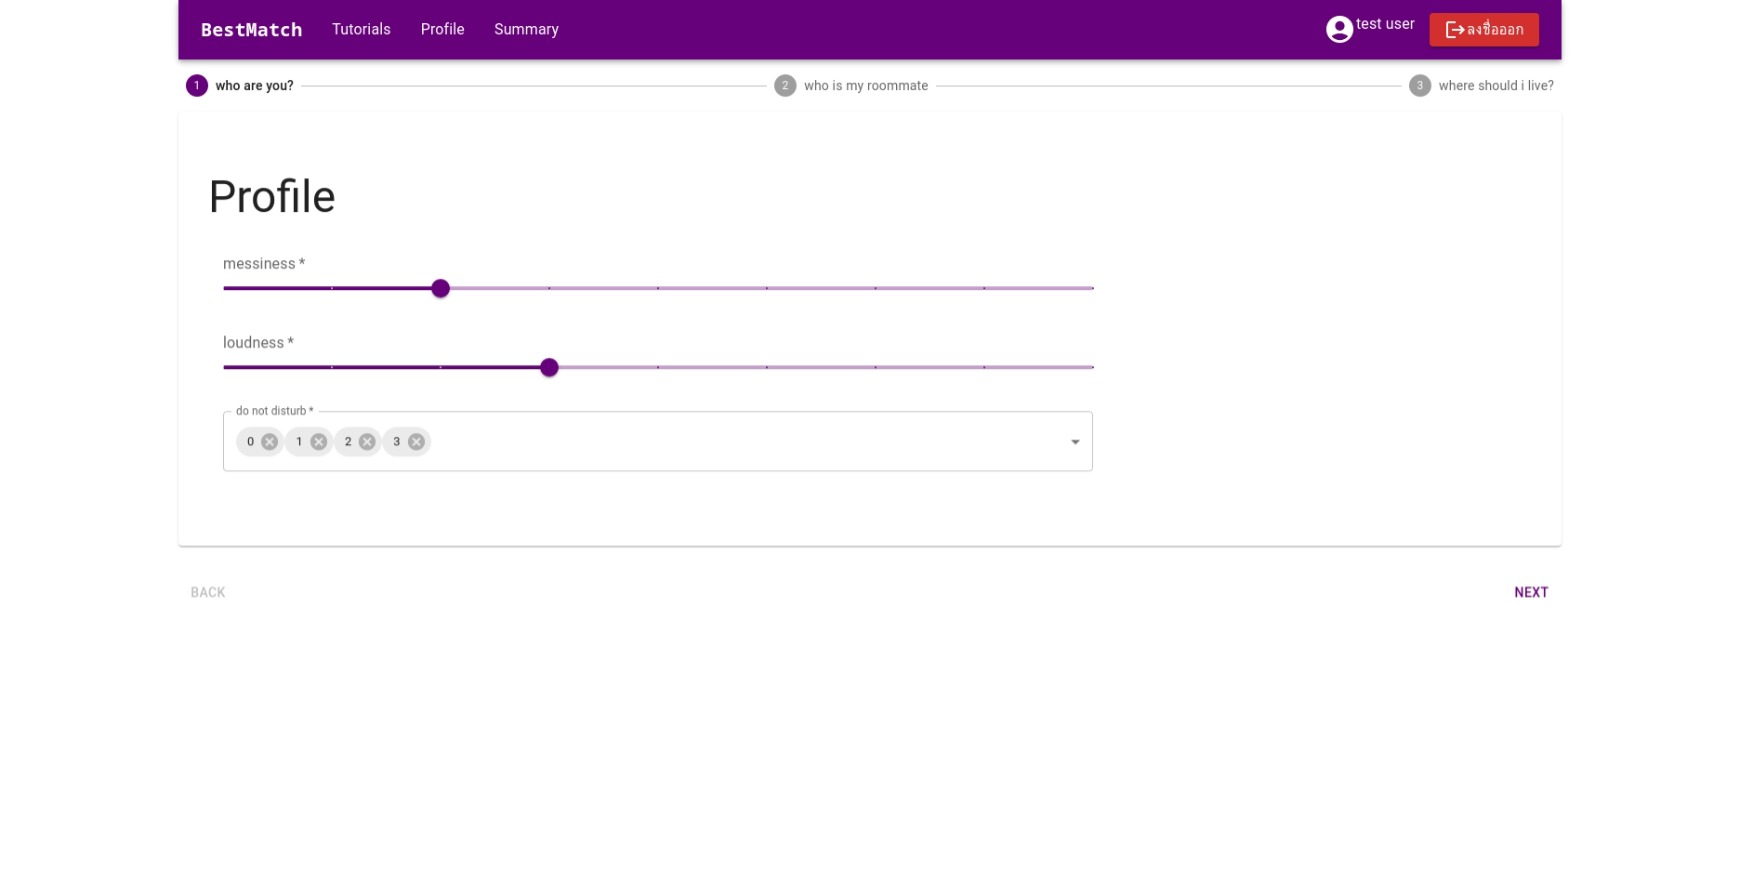
\includegraphics[width=\linewidth]{photo/web/student/profile-def.jpeg}
  \end{center}
  \caption{หน้าระบุ profile ของผู้ใช้}
\end{figure}
\newpage

หลังจากนั้นระบุ preference ของรูมเมทที่ต้องการ เมื่อเสร็จแล้วกดปุ่ม "NEXT"
\begin{figure}[h]
  \begin{center}
    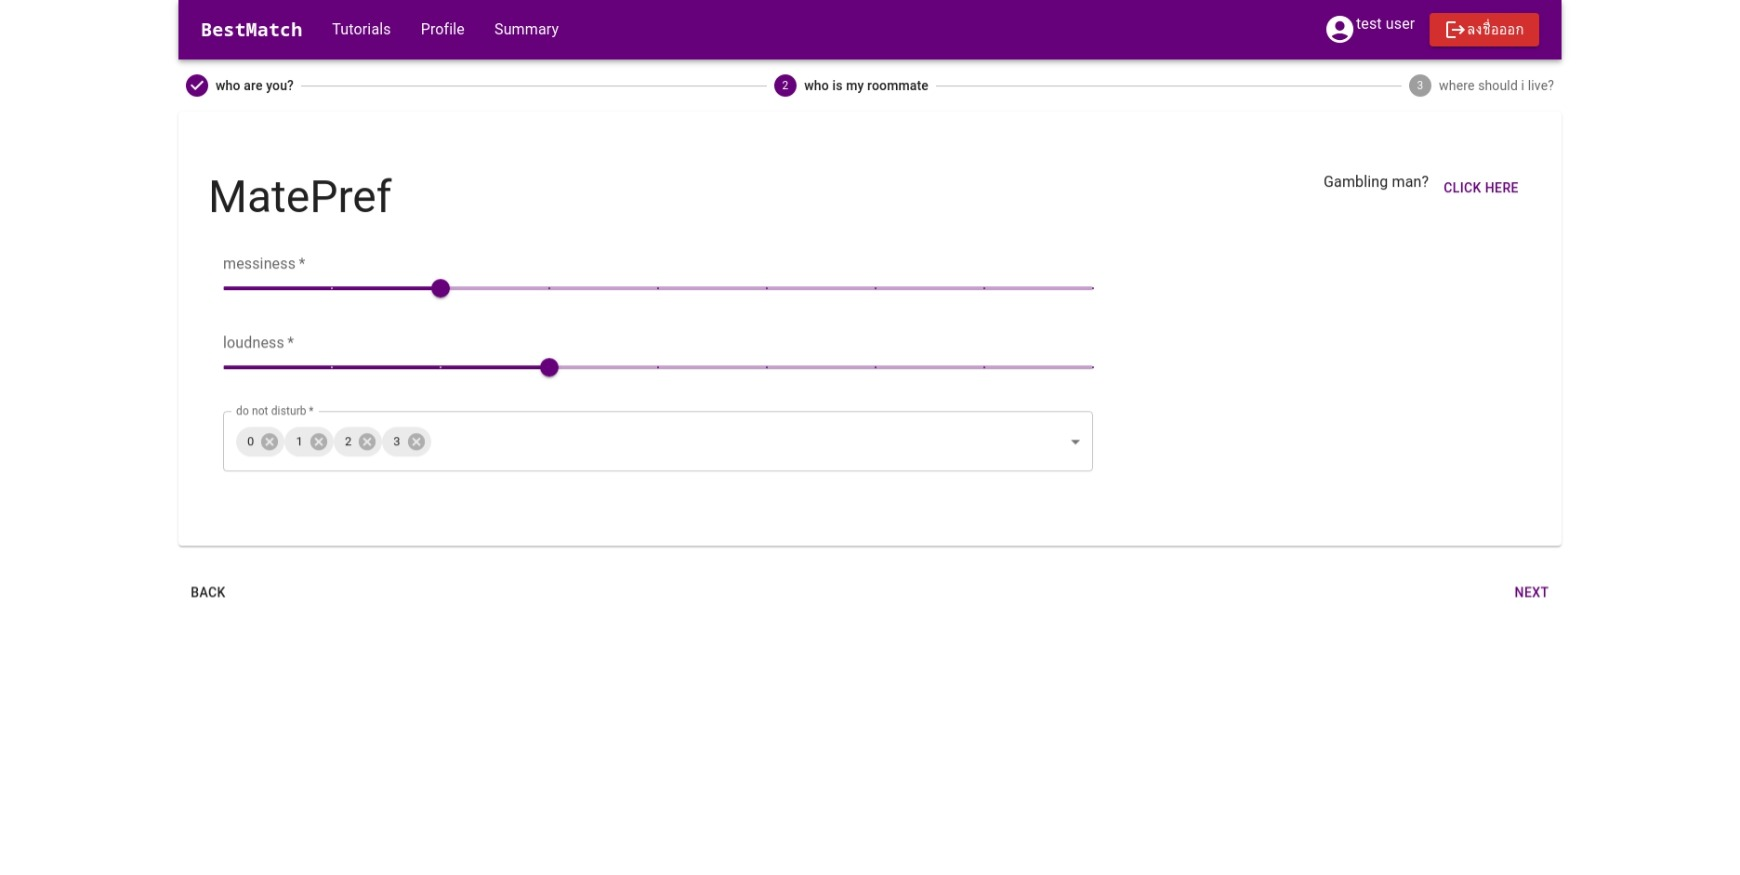
\includegraphics[width=\linewidth]{photo/web/student/mate-def.jpeg}
  \end{center}
  \caption{หน้า preference ของรูมเมท}
\end{figure}
%
\newline
โดยหากผู้ใช้ไม่อยากระบุ preference ของรูมเมทก็สามารถกด "CLICK HERE" ได้
\begin{figure}[h]
  \begin{center}
    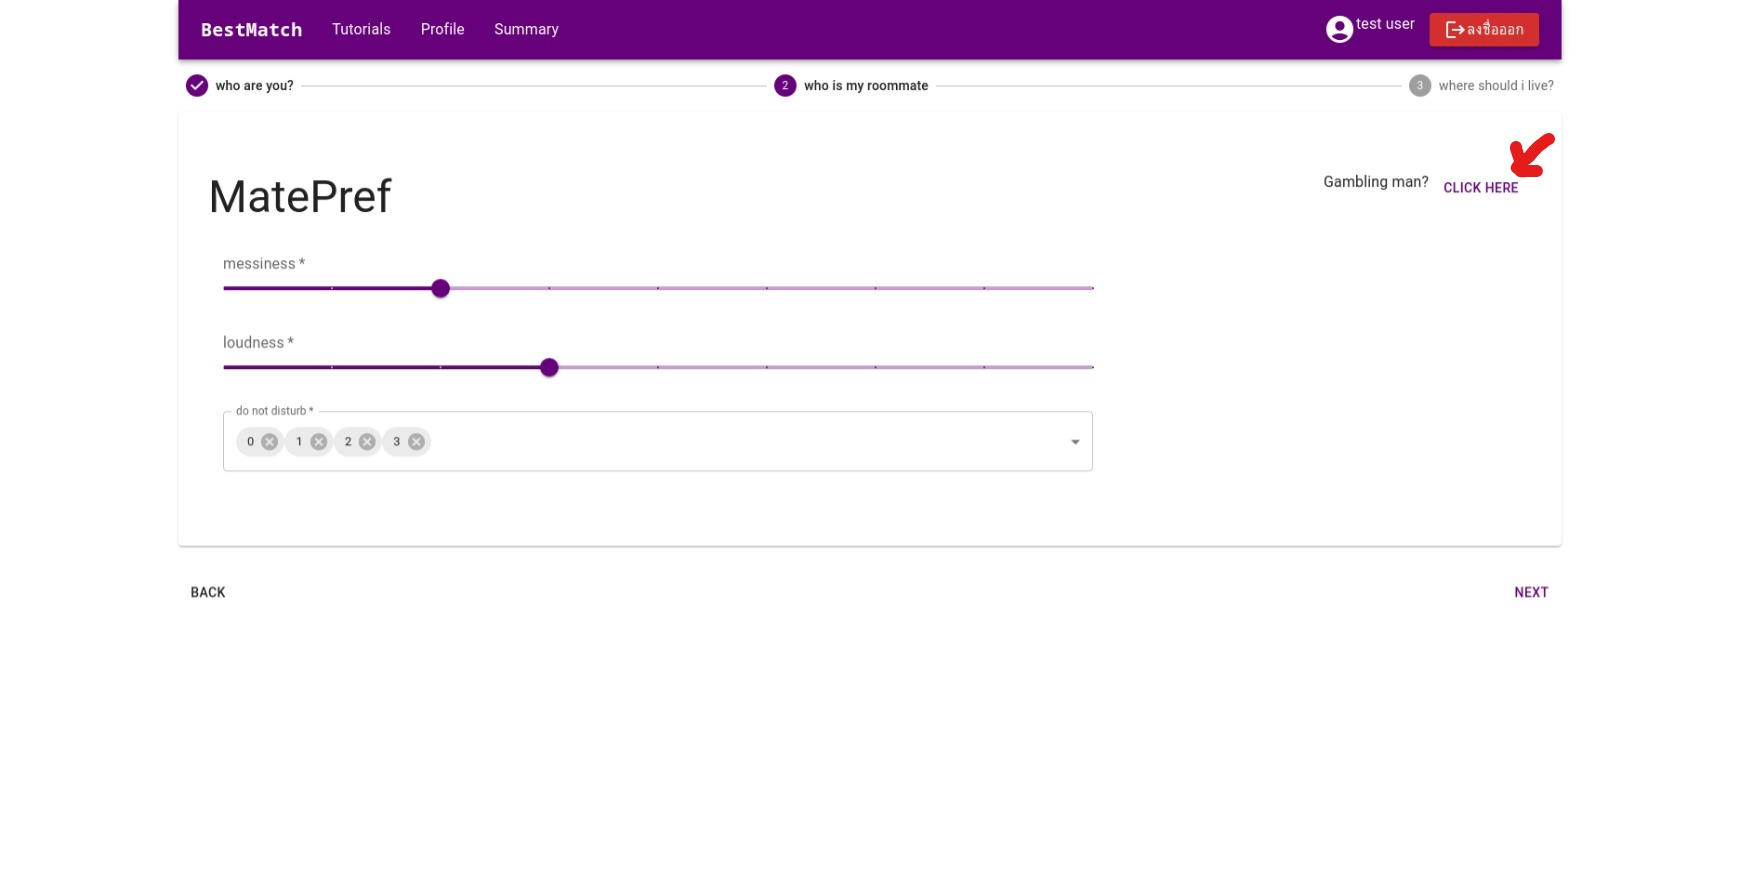
\includegraphics[width=\linewidth]{photo/web/student/mate-gambler.jpeg}
  \end{center}
  \caption{รูปตัวอย่างแสดงตำแหน่งปุ่ม "CLICK HERE" ของหน้า preference ของรูมเมท}
\end{figure}
\newpage

หลังจากนั้นระบุ preference ของห้อง และ หอพักที่ต้องการ เมื่อเสร็จแล้วกดปุ่ม "NEXT"
\begin{figure}[h]
  \begin{center}
    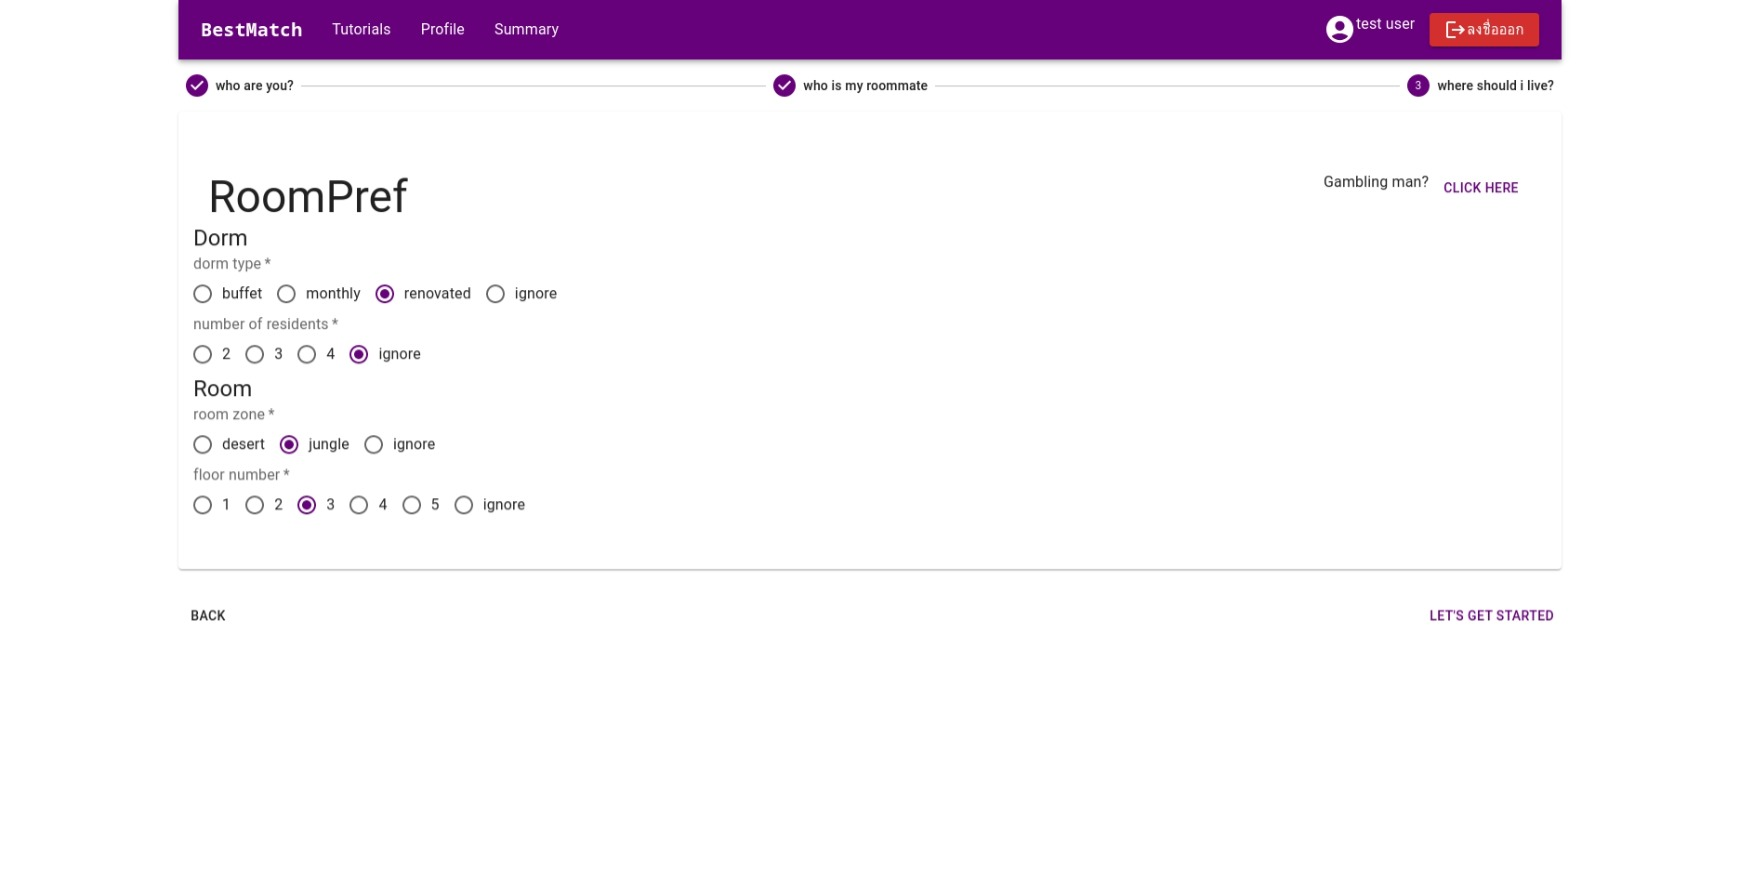
\includegraphics[width=\linewidth]{photo/web/student/dorm-def.jpeg}
  \end{center}
  \caption{หน้า preference ของหอพัก}
\end{figure}
%
\newline
โดยหากผู้ใช้ไม่อยากระบุ preference ของหอพัก และห้องพักก็สามารถกด "CLICK HERE" ได้
\begin{figure}[h]
  \begin{center}
    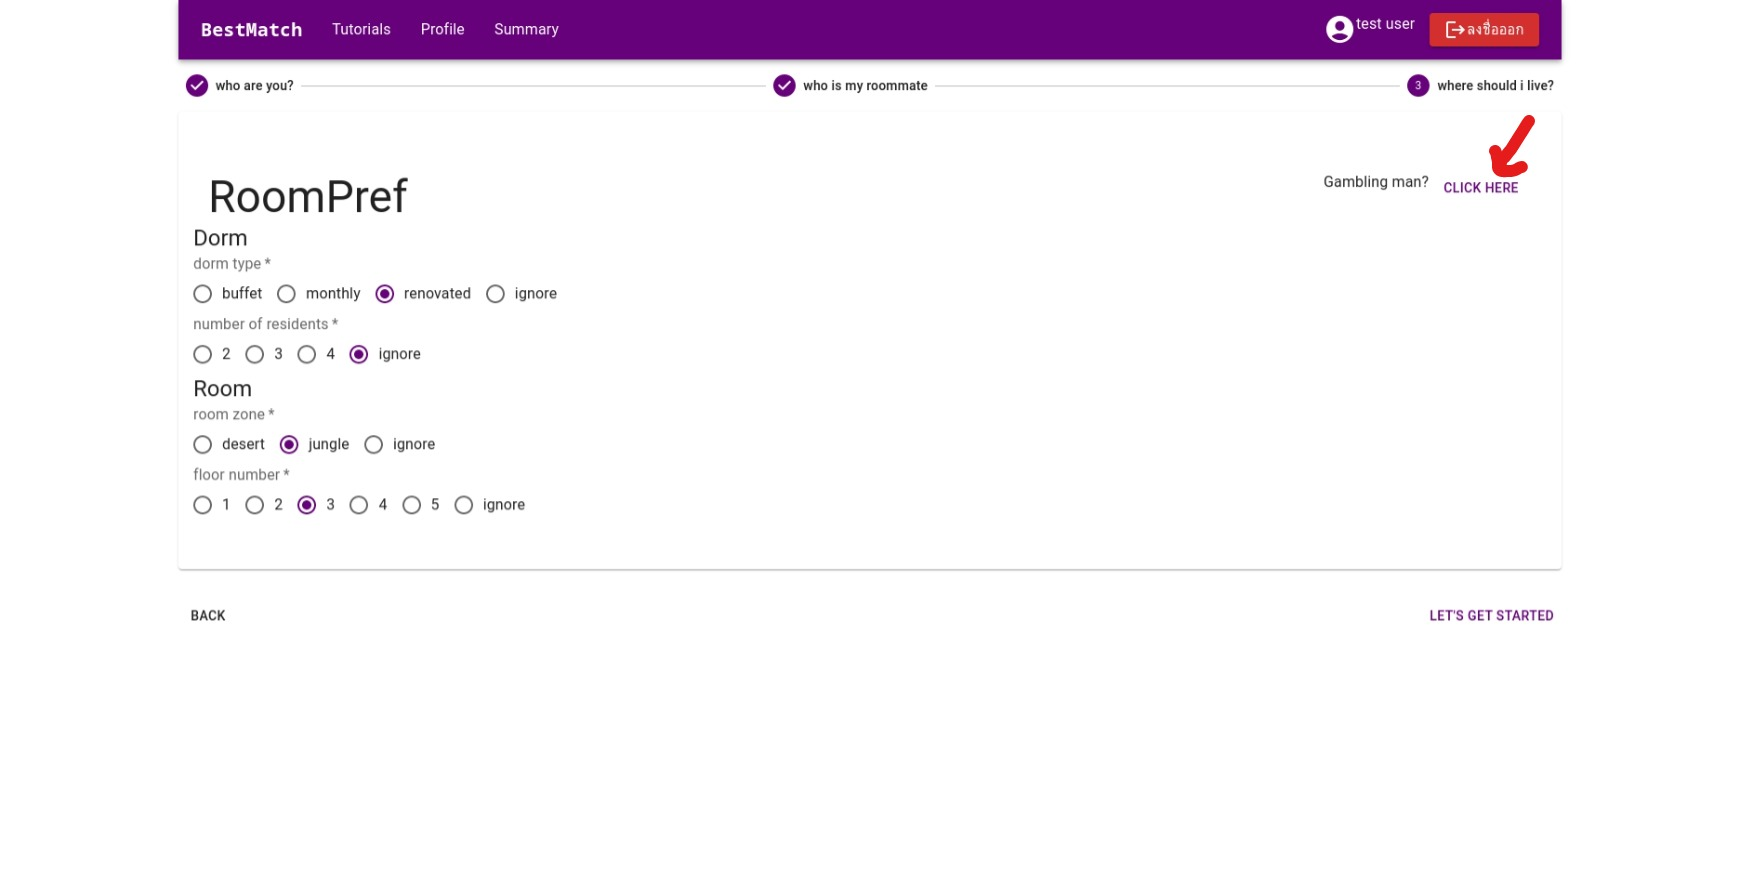
\includegraphics[width=\linewidth]{photo/web/student/dorm-gambler.jpeg}
  \end{center}
  \caption{รูปตัวอย่างแสดงตำแหน่งปุ่ม "CLICK HERE" ของหน้า preference ของหอพัก}
\end{figure}
\newpage
%
% หลังจากนั้นจะเป็นหน้าที่ให้ผู้ใช้เลือกว่าจะเอาโปรไฟล์สมมุติ โปรไฟล์ไหนสำหรับการ finetune
% \begin{figure}[h]
%   \begin{center}
%     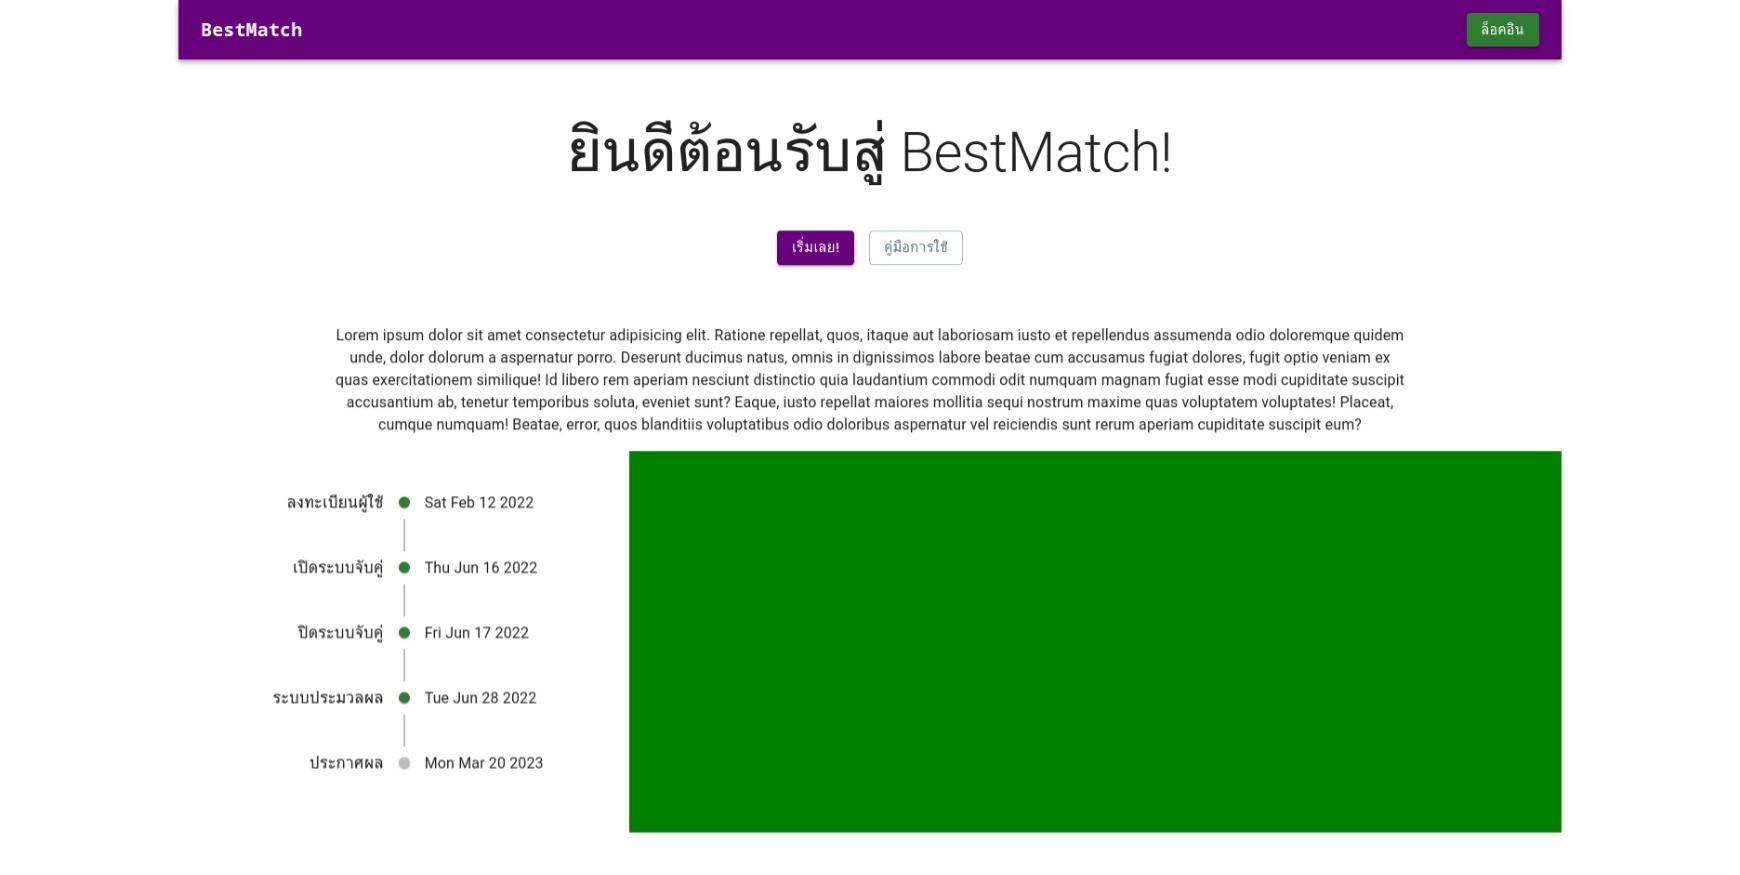
\includegraphics[width=\linewidth]{photo/web/student/home.jpeg}
%   \end{center}
%   \caption{หน้า Home}
% \end{figure} 
% %
% \newline
% หากผู้ใช้พึงพอใจกับการ finetune แล้วสามารถกลับหน้า Home ได้โดยคลิกที่ไอคอน "BESTMATCH"
% \begin{figure}[h]
%   \begin{center}
%     
\includegraphics[width=\linewidth]{photo/web/student/icon-btn.jpeg}
%   \end{center}
%   \caption{รูปตัวอย่างแสดงตำแหน่งปุ่มไอคอน "BESTMATCH"}
% \end{figure}
% \newpage
%
ซึ่งผู้ใช้สามารถตรวจสอบโปรไฟล์ของตนเองได้ที่หน้า Profile
\begin{figure}[h]
  \begin{center}
    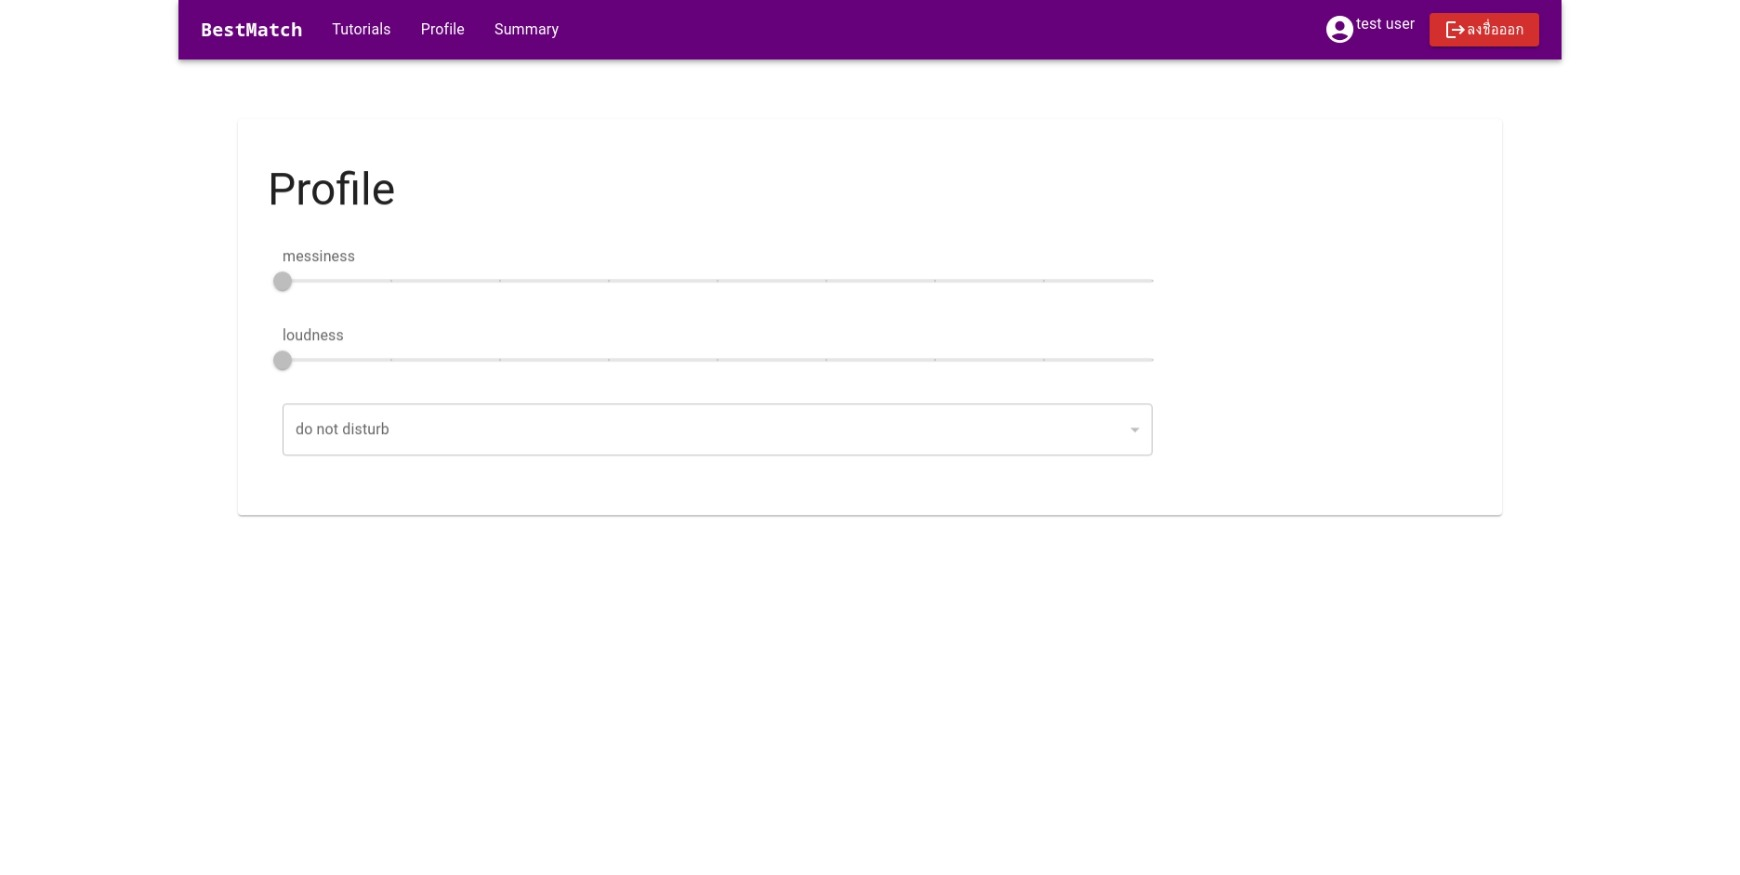
\includegraphics[width=\linewidth]{photo/web/student/profile.jpeg}
  \end{center}
  \caption{หน้า Profile}
\end{figure}
%
\newline
และสามารถตรวจสอบรูมเมทที่คาดว่าจะได้จากการจับคู่ที่หน้า Summary
\begin{figure}[h]
  \begin{center}
    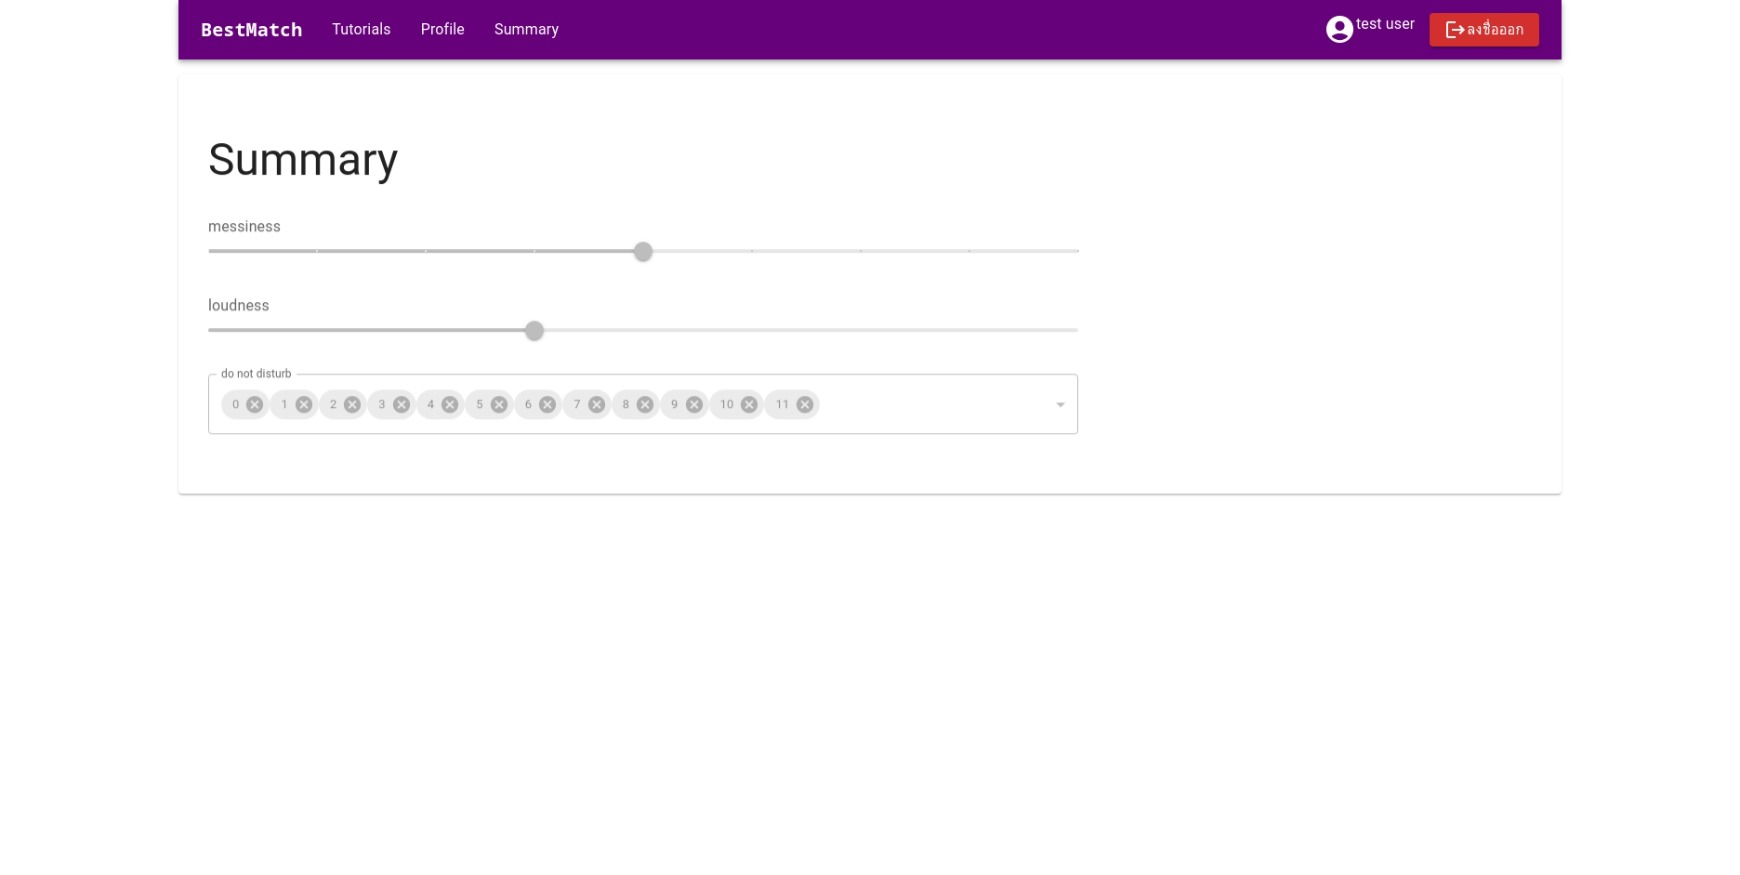
\includegraphics[width=\linewidth]{photo/web/student/summary.jpeg}
  \end{center}
  \caption{หน้า Summary}
\end{figure}